\subsection{Bild auf eine Karte zeichnen}\label{bilder} 
Um ein Bild auf eine Karte zeichnen zu können, muss das Bild als \textsf{pyplot.image} vorliegen. Dies kann man mit Hilfe der \textsf{PIL} erreichen. Da \textsf{matplotlib.image} eine Funktion \textsf{pil\_to\_array(Pilimage)} zur Verfügung stellt. Beim Zeichnen von Bildern muss man beachten das sie über die ganze Karte gezeichnet werden. Die Funktion um ein Bild zu zeichnen ist \textsf{imshow(X, cmap=None, norm=None, aspect=None, interpolation=None, alpha=None, vmin=None, vmax=None, origin=None, extent=None, shape=None, filternorm=1, filterrad=4.0, imlim=None, resample=None, url=None, hold=None, **kwargs)}. Sie bekommt in \textsf{X} ein Bild als Pixelmatrix übergeben. Die anderen Parameter werden einfach an \textsf{pyplot.imshow()} weitergegeben. Die Parameter \textsf{extent} und \textsf{origin} werden automatisch so gesetzt, das das Bild über die ganze Karte gemalt wird.\\
Mit der Funktion \textsf{warpimage(image='bluemarble', scale=None, **kwargs)} kann man ein Hintergrundbild laden. Dieses Bild muss allerdings den ganzen Globus abdecken. Im Parameter \textsf{image} kann man einen Filenamen oder eine URL angeben. Sollte eine URL angegeben sein wird das Bild von der entsprechenden Seite als temporäre Datei herunter geladen. Dabei muss die URL mit \textsf{http} anfangen. Sollte nichts angegeben sein wird ein \textsf{blue marble next generation} Bild von  
\textsf{http://visibleearth.nasa.gov/} genommen.\\
Mit der Funktion \textsf{wmsimage(server, xpixels=400, ypixels=None, format='png', verbose=False, **kwargs)} kann man ein Hintergrundbild von einem WMS Server laden und zeichnen. Damit diese Funktion funktioniert muss die Karte mit dem passenden Parameter \textsf{epsg} erstellt worden sein, oder die Projektion \textsf{cyl} gewählt sein.\\
Mit der Funktion \textsf{arcgisimage(server='http://server.arcgisonline.com/ArcGIS', service='ESRI\_Imagery\_World\_2D', xpixels=400, ypixels=None, dpi=96, verbose=False, **kwargs)} kann man ein Hintergrundbild von einem ArcGIS Server laden und darstellen. Mit dem Parameter \textsf{service} kann man einstellen welcher Art das Bild sein soll. Um diese Funktion benutzen zu können muss beim erstellen der Karte der Parameter \textsf{epsg} passend gesetzt worden sein, oder die Projektion \textsf{cyl} gewählt sein. Mit den Parametern \textsf{xpixels} und \textsf{ypixels} kann man die Anzahle Pixel in der Breite und Höhe einstellen. Sollte \textsf{ypixels} nicht gesetzt sein wird die Anzahl Pixel in der Höhe von der Anzahl Pixel in der Breite berechnet, so dass das Seitenverhältnis beibehalten bleibt.\\
Mit der Funktion \textsf{bluemarble(ax=None, scale=None, **kwargs)} kann man ein \textsf{blue marbel} Bild als Hintergrund malen. Mit Hilfe des Parameters \textsf{scale} kann man die Pixel Anzahl reduzieren, damit das Bild schneller geladen werden kann. Die Standardgröße des Bildes ist 5400x2700.\\
\lstinputlisting{/Users/student/seminar/bsp/bspmarble.py}
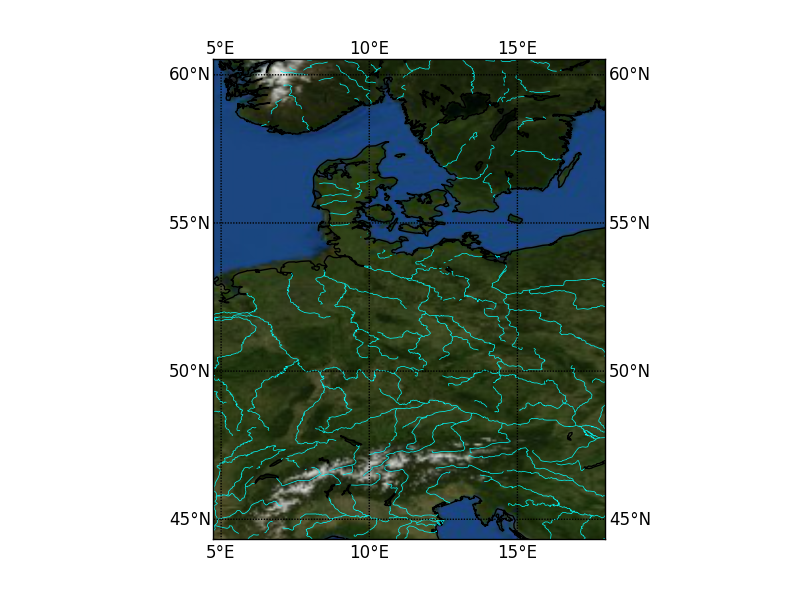
\includegraphics[scale=0.4]{/Users/student/seminar/bsp/bspmarble}